\documentclass[11pt]{article}
\usepackage{graphicx}
\usepackage{caption}
\usepackage[multiple]{footmisc}
\usepackage{cleveref}
\usepackage{lipsum}
\usepackage{wrapfig}
\usepackage{subfig}
\usepackage{tabularx}
\usepackage[T1]{fontenc}
\usepackage{amsmath}
\usepackage{fixltx2e}
\usepackage[font=scriptsize,labelfont=bf]{caption}
\crefformat{footnote}{#2\footnotemark[#1]#3}
%Gummi|065|=)
\title{\textbf{Action selection - Guthrie Model}}
\author{Bhargav Teja Nallapu}
\begin{document}

\maketitle

\listoffigures

\section{Context}
Basal Ganglia (BG) are known to be responsible for decision making and learning in a changing environment.\emph{Gurthrie et al,} 2013 proposes a computational model for two-level action selection with two parallel functional loops each for cognitive and motor decision making. Each loop consists of a positive feedback direct pathway and a negative feedback hyper-direct pathway  via the subthalmic nucleus to globus pallidus. In addition to the cognitive and motor ensembles, there are associative areas in cortex and striatum. The divergence and reconvergence of the direct pathway facilitates the information transfer between the cognitive and motor loops and hence providing a bias to the motor decision.
\par 

\section{Materials and Methods}

\textbf{\emph{Task}}. The task used in the model to demonstrate action selection is a probabilistic learning task as described in Pasquereau et al. 2007. 4 target shapes are associated with different reward probabilities.
A trial is a time period in which two of the four possible shapes are randomly chosen and presented (to the subject, \emph{the model} in this case) at two random positions (of the possible positions - up, right, down and left). By the end of trial period, a choice is made by the \emph{model} and the reward is presented (corresponding to the reward probability of the chosen shape). In a single independent trial, the cognitive decision (shape of the cue) and motor decision (direction of position) could be independent of each other.  
\par
\textbf{\emph{Experiment setup}}. The first 500 ms of the trial is for settling of the model. Then the two random cues are presented. A trial is considered to be successful if a decision is made by the \emph{model}, irrespective of the reward received. At any decision-making level of the \emph{model}, each of the four cue shapes and each of the four motor movement directions is represented one unit (neuron) each. Thus in a given trial, when two cue shapes are presented at two different positions, two cognitive, two motor and two associative (wherever applicable) neurons are activated.  The task is run for a session, a number of trials.
\par
\textbf{\emph{Learning}}. The \emph{model} incorporates learning by taking the reward received in each trial into account forming a type of actor-critic network (Barto 1995). The learning changes the synaptic weights for the cortico-striatal gains over trials, particularily between the cognitive channels. 
\begin{wrapfigure}{r}{0.5\textwidth}\vspace*{-1\baselineskip}%
  \begin{center}
  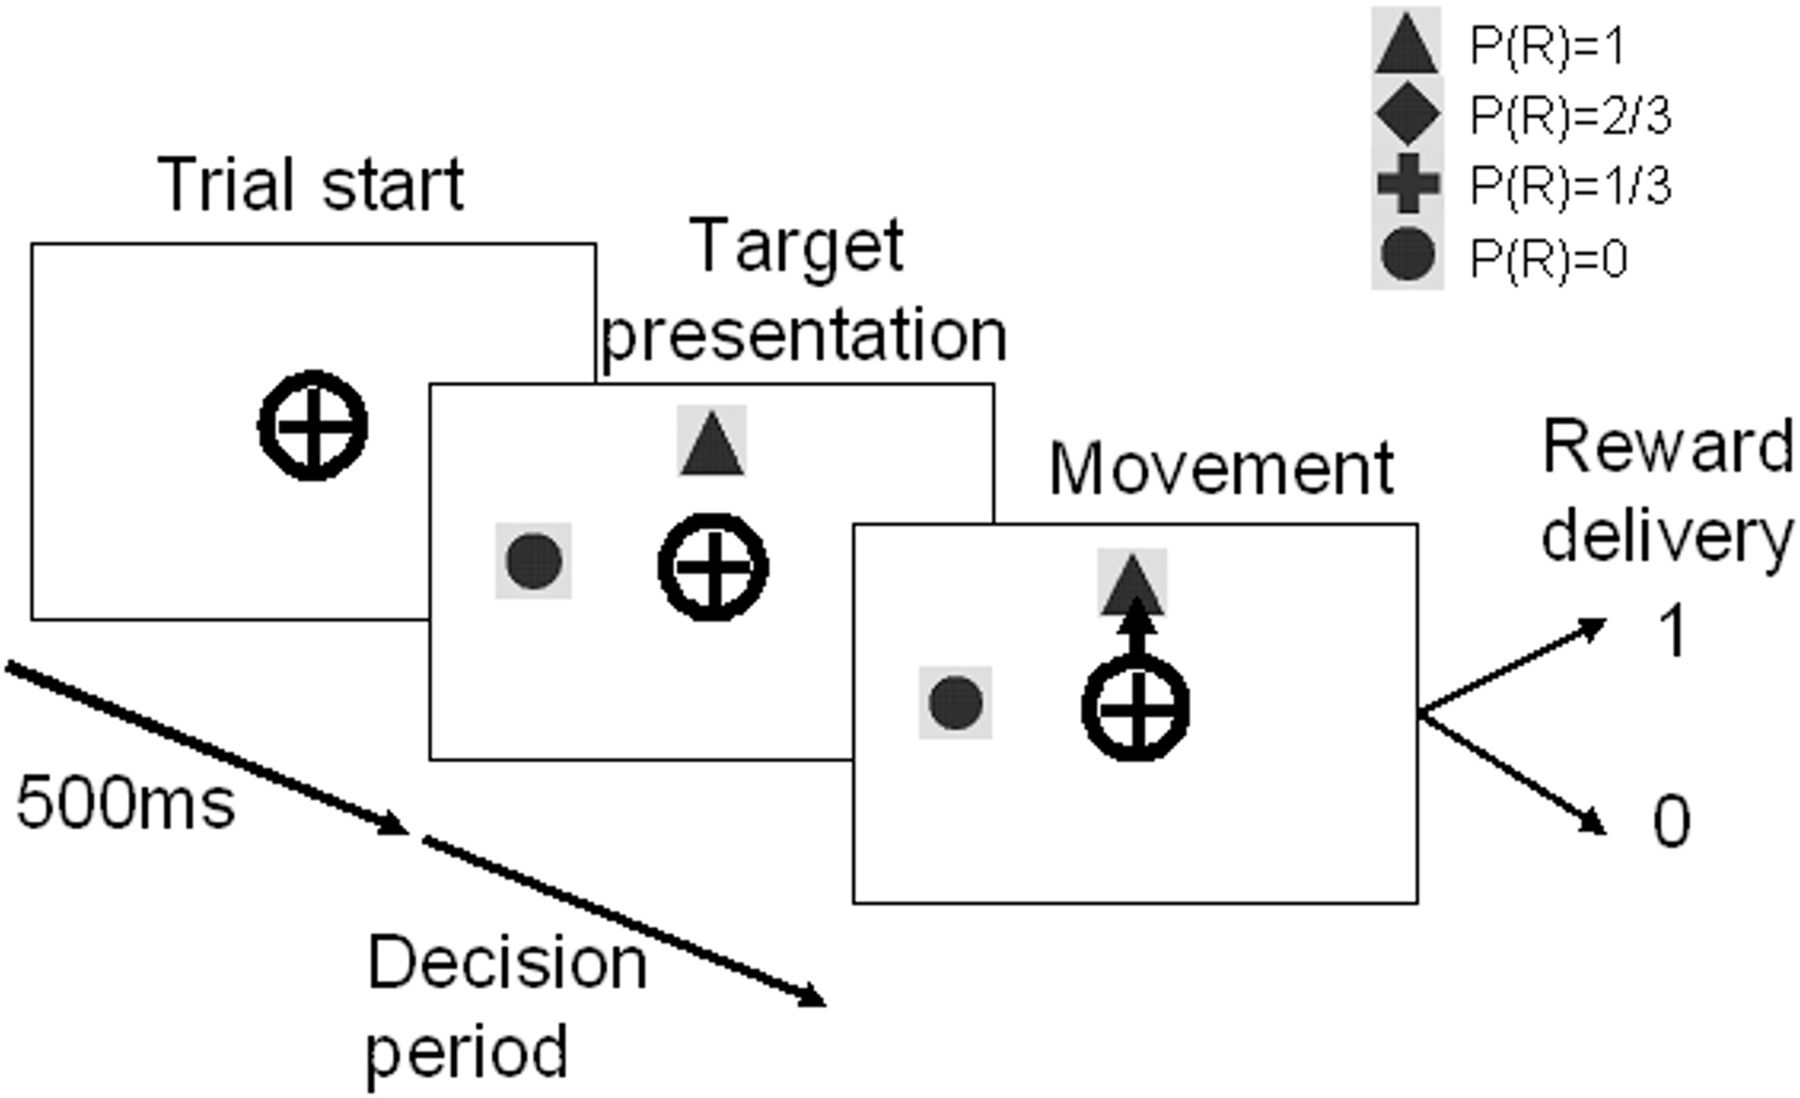
\includegraphics[width=0.48\textwidth]{two-armed.jpg}
  \end{center}
  \caption[2-armed bandit task in Guthrie model]{2-armed bandit task in Guthrie model, as described in Pasquereau et al. 2007. The \emph{model} has to make a cognitive decision about the shape and a motor direction decision, ideally towards the position of selected shape.}
\end{wrapfigure} The \emph{model} design allows bidirectional information transfer between loops, a consequence of which was that, in early trials, a direction could be selected before a shape leading to a motor bias of cue selection(Fig. 1). However, after multiple trials , the \emph{model} begins to consistently make cognitive decision before the motor decision in each trial and most frequently the motor decision towards the position of the more rewarding cue shape.\par

Accounting to the major characteristics of the Guthrie \emph{model}, an elobarative and reproducible computational model\footnote{http://www.labri.fr/perso/nrougier/downloads/ReproducibleScience.pdf} has been developed by \emph{Meropi Topalidou}\footnote{\label{imn}Institute of Neurodegenerative Diseases - Bordeaux}\footnote{\label{inria}INRIA Bordeaux SUD-OUEST}, \emph{Arthur Leblois}\footnote{Laboratory of Neurophysics and Physiology Universite Paris Descartes}, \emph{Thomas boraud}\cref{imn}, \emph{Nicolas P. Rougier}\cref{imn}\cref{inria}. This model reproduces the distinct activity of the chosen cue shape and the direction of chosen position (Fig. 2).\par

\textbf{\emph{Neuronal dynamics}}. This model uses the same simplistic neuronal rate model as in Leblois et al. (2006) as used by the Guthrie \emph{model} to focus on the network dynammics. Within each structure, each neuron (in each channel of any loop) is modeled as a single rate neuron with the equation:
\begin{equation}
\tau \cfrac{dm}{dt} = -m + I_s + I_{Ext} - T
\end{equation}
decay time constant of the synaptic input $\tau$, negative values of activation, \emph{m} and threshold of the neuron \emph{T} are set to respective constant values as per the Guthrie's \emph{model}. $I_{Ext}$ is an external input representing the sensory visual salience of the cue, which is unchanged thoughout the process of learning.

\begin{figure}[ht]
  \centering
  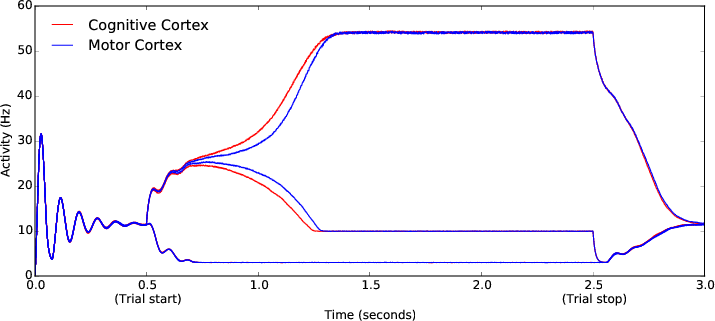
\includegraphics[width=\textwidth]{figure-1.png}
  \caption[Activity of the channels in both cognitive and motor cortex varying with the trial time]{Activity (Hz) of all the channels in both cognitive and motor cortex varying with the trial time (seconds). The cognitive and motor activity corresponding to the cues which are not presented is constant(nearly zero). Of the 2 cues presented, the activity can be seen changing at a point (when decision is made). Also, it can be seen that for the cue whose activity increased (implying the cue has been chosen), cognitive activity (in red) rises before the motor activity (in blue) implying that the cognitive decision has been made before the motor decision.}
\end{figure}
When the \emph{model} is presented over a session of many trials (120 in this case), the two cue shapes in each trial are randomly chosen from the four. And it is made sure all the pairwise combinations of the shapes appear equal number of times throughout the session (6 combinations, 20 times each). Towards the last trials of the session, the model having learnt, the motor decision is biased towards the position of the cue shape which has been more rewarding from the beginning of the session. Many such independent sessions are run (in this case, 250). The performance of the model is measured by checking if the model made a motor position decision corresponding to the best rewarding cue shape of the two presented. This is measured as an average of each trial over different sessions. It is also reproduced that the mean performance of the \emph{model} reaches close to 1 (Fig. 3), implying that after learning, the \emph{model} most certainly selects the direction of the most rewarding cue in a given trial.
\begin{figure}[ht]
  \centering
  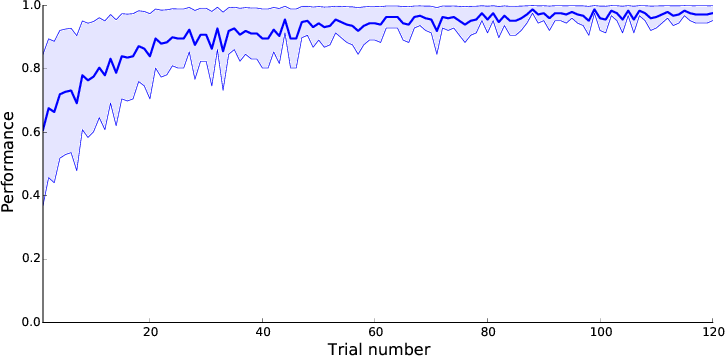
\includegraphics[width=\textwidth]{figure-2.png}
  \caption[Performance of the model over various simulations]{Performance of the model over various simulations.Each simulation consisting of 120 trials, is independent of one another. The learning that happens over 120 trials in a simulation is reset by resetting weights at the beginning of each simulation. A decision is considered correct if the motor decision made is in the direction in which the more rewarding cue is present. The performance is an average over all the simulations for each trial. It can seen that as the learning happens upto 120 trails, model tends to perform nearly accurate i.e, selecting the more rewarding cue almost every trial}
\end{figure}


\section{Developments}
\subsection{Learning in cortico-striatal motor channels}
As mentioned in \emph{Learning, Materials and Methods}, the \emph{model} learns only in the cognitive channels of the cortico-striatal areas, assuming the reward probability os associated to the cognitive aspect, i.e, the shape of the cue. The \emph{model} is replicated, and learning is incorporated between the cortico-striatal motor channels. In every trial of the session, the weights of the cortico-striatal motor channels (position of the cue) are also adjusted besides that of cognitive channels upon the reward given. It can be observed that because of the learning, the synaptic weights are adjusted such that the weight of the channels associated to the more rewarding cue shapes is distintly more than the others (Fig.4).  \par
\begin{figure}[!hb]
  \begin{center}
\def\tabularxcolumn#1{m{#1}}
\begin{tabularx}{\linewidth}{@{}cXX@{}}
\begin{tabular}{cc}
\subfloat[Cognitive channel weights]{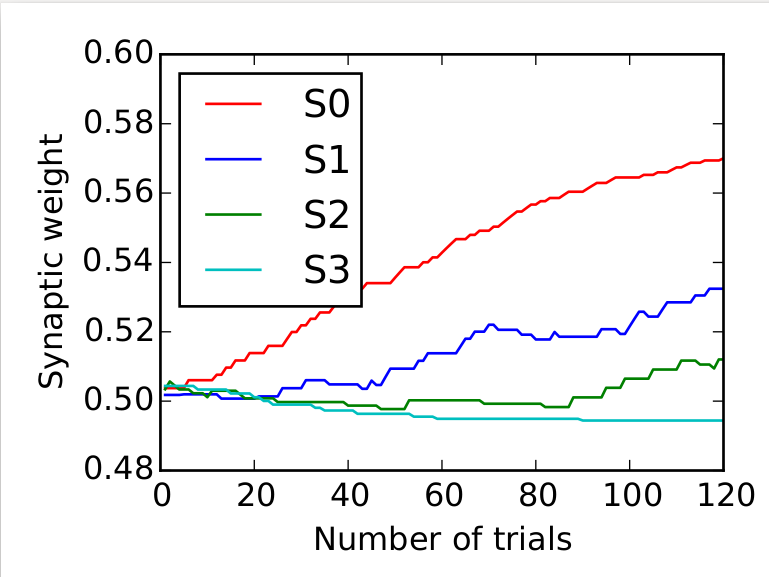
\includegraphics[width=0.45\textwidth]{SC1.png}} 
   & \subfloat[Motor channel weights]{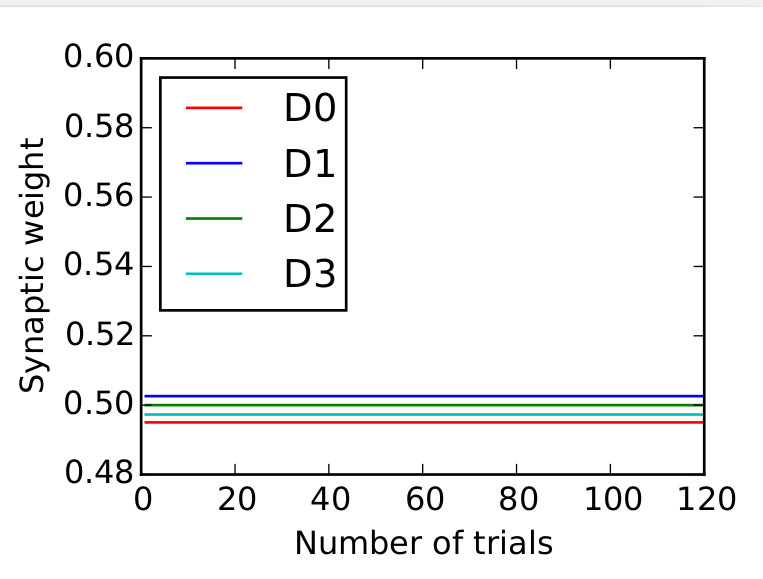
\includegraphics[width=0.45\textwidth]{SM1.png}}\\
\subfloat[Cognitive channel weights]{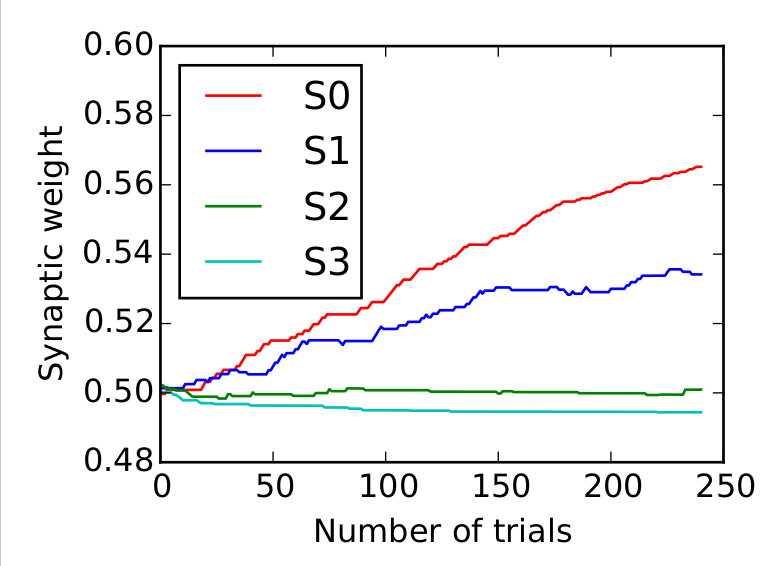
\includegraphics[width=0.45\textwidth]{SC2.png}} 
   & \subfloat[Motor channel weights]{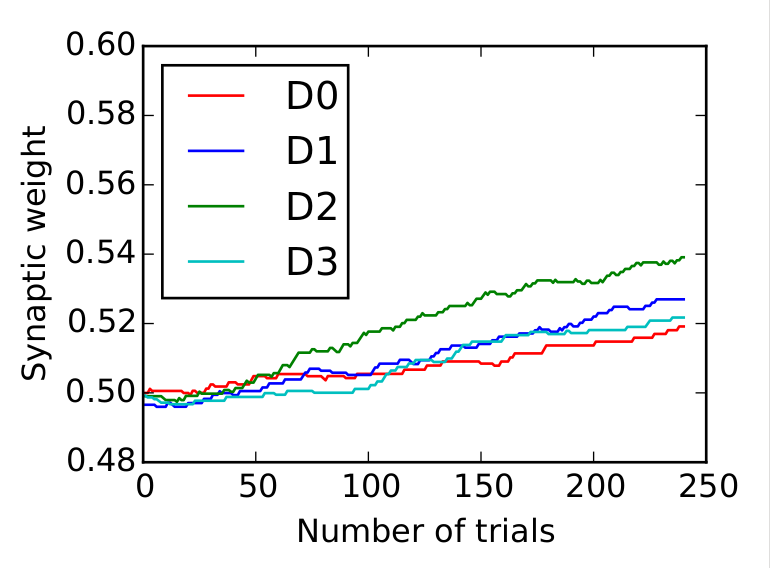
\includegraphics[width=0.45\textwidth]{SM2.png}}
\end{tabular}
&
\end{tabularx}
\caption[Synaptic cortico-striatal weights]{Synaptic cortico-striatal weights changing over trials. 4(a)\&(b) as in the original \emph{model} with learning only in cortico-striatal cognitive channels. Weights of channels are shown in different colors. S0,...S3 represent weights of channels associated with each of four cue shapes whereas D0,...D3 represent that of each position where cues could be shown. 4(a) shows that eventually after learning, the weight of one channel that of highly rewarding cue shape is distinctly higher than that of other cue shapes. As there is no learning in motor channels, the motor channel weights are unchanged as in 4(b). After modifying the \emph{model} to add learning in cortico-striatal motor channels, 4(c) shows that the cognitive channels still learn as expected, increasing the weights as per the reward associated with the cue shape. At the same time, the motor channel weights are observed to be changed 4(d). Although reward given was not associated to the position of the cue presented, the \emph{model} attributes certain positions to be rewarding by increasing motor channel weights.}\label{weights}
  \end{center}
\end{figure}
\begin{figure}[ht]
  \centering
  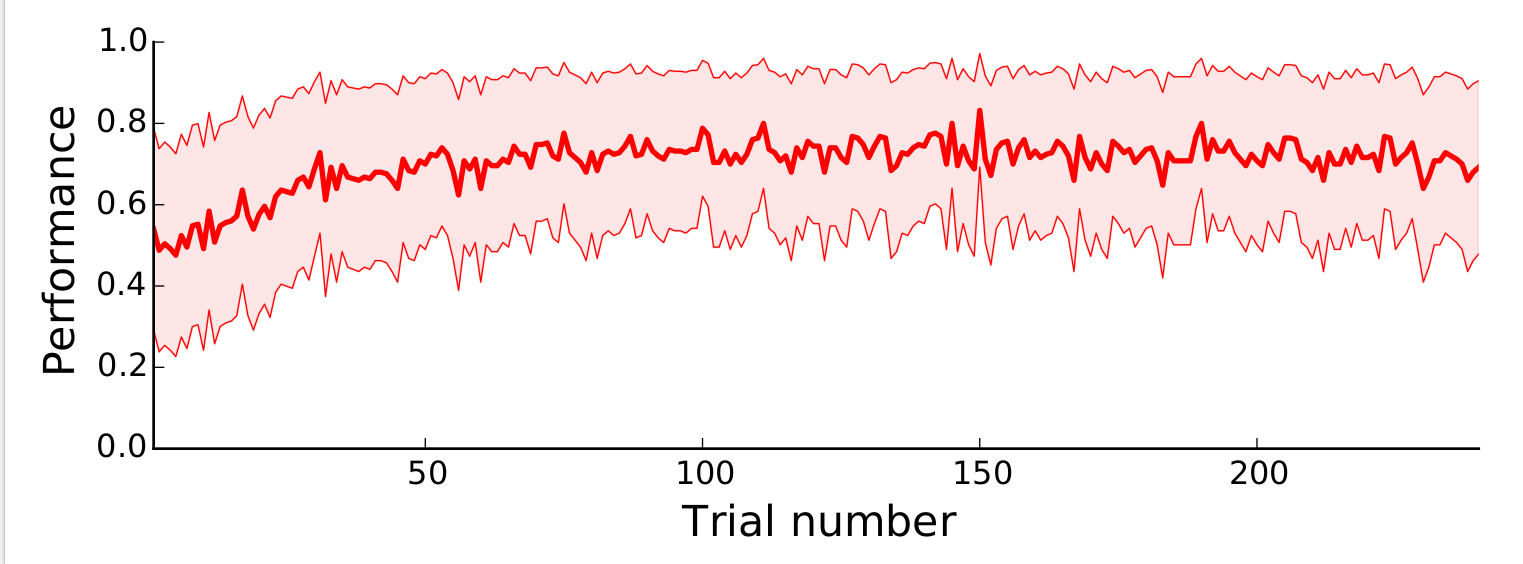
\includegraphics[width=\textwidth]{P2.png}
  \caption[\emph{Model} performance in the presence of motor channel learning]{\emph{Model} performance in the presence of motor channel learning. As it can be compared to Fig.3, the performance is found to be reduced when the cortico-striatal motor channels learn through the session. }
\end{figure}

\textbf{\emph{Reduced performance}}. With the addition of motor channel learning, the \emph{model} is run through 250 simulations, each with 120 trials. The learning rates , cortico-striatal gains and other parameters are set as per the original \emph{model}. Besides the updated weights of motor channel, a reduced mean performance is observed when compared to the \emph{model}'s mean performance in the absence of motor channel learning (Fig.5).\par

\textbf{\emph{Faster motor decision}}. The original \emph{model} with learning only in the cognitive channels, shows that motor decision time is consistently higher than the cognitive decision time in each trial, suggesting that the best shape is chosen and thus a motor decision is taken depending on the position of chosen shape. However, with the addition of learning in motor channel to the \emph{model}, motor decision did not occur consistently after the cognitive decision implying that motor decision is hardly biased by the cognitive decision (chosen shape) (Fig. 6) and thereby affecting the overall performance. \par
\begin{figure}[ht]
  \begin{center}
\def\tabularxcolumn#1{m{#1}}
\begin{tabularx}{\linewidth}{@{}cXX@{}}
\begin{tabular}{cc}
\subfloat[Original model]{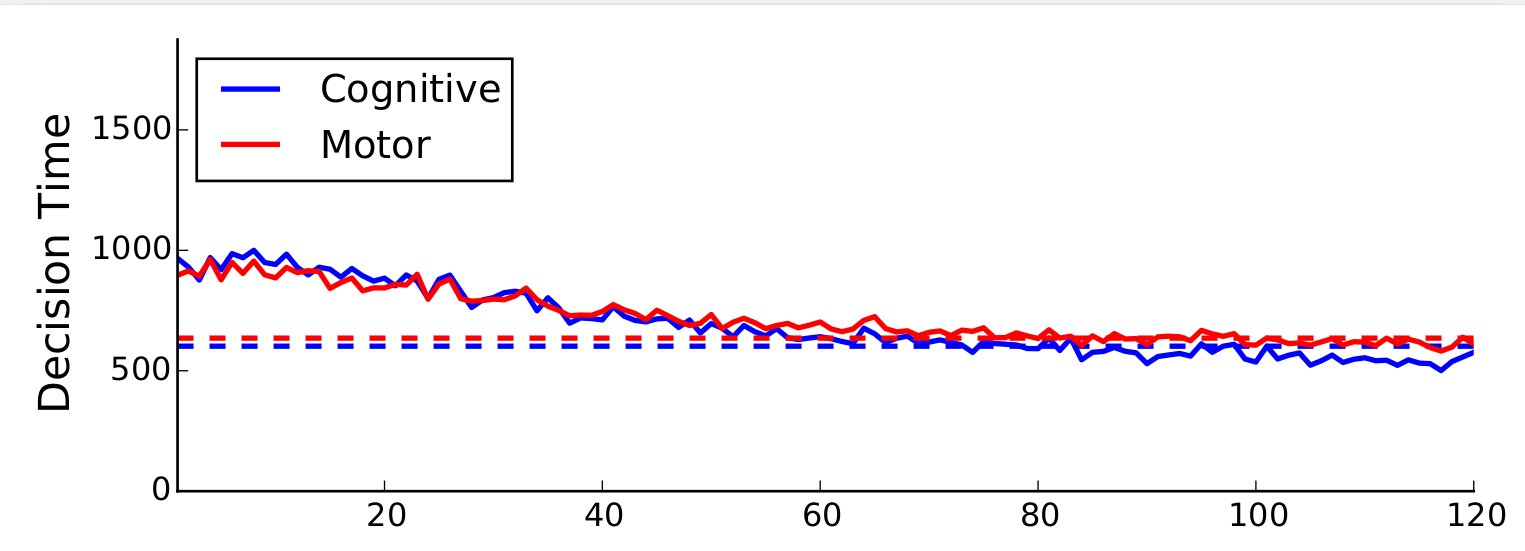
\includegraphics[width=0.9\textwidth]{T1.png}} \\
\subfloat[Model with learning in motor channels]{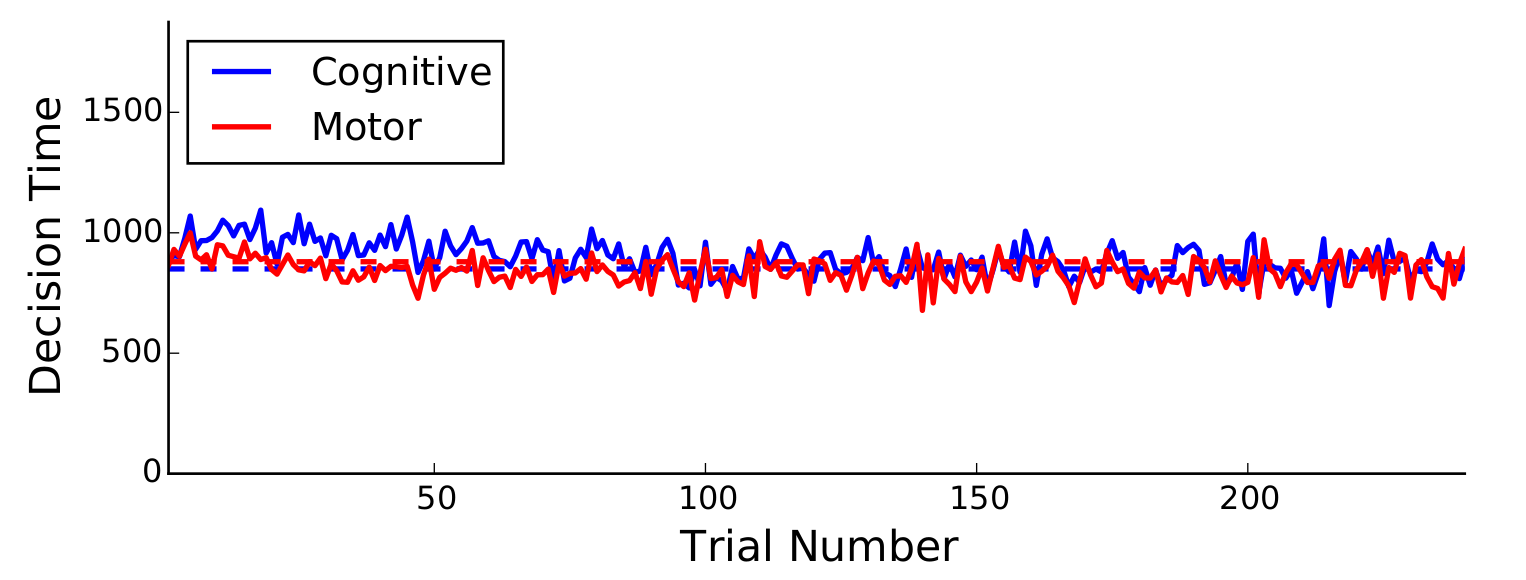
\includegraphics[width=0.9\textwidth]{T2.png}}

\end{tabular}
&
\end{tabularx}
\caption[Decision times for each trials]{Decision times for each trial. The lines with dash represents the average decision time across all the trials. In the original model (a), when there is no learning in the motor channels, the motor decision time (in red) is more than the cognitive decision time (in blue), towards the ending trials. When the learning in motor channels is introduced (b), there is no such consistency of motor decision time observed, which implies motor decision (direction of position) was not necessarily biased by the cognitive decision (cue shape)}\label{decision times}
\end{center}
\end{figure}

\subsection{Non-simultaneous cue presentation}
In the task presented in the original \emph{model}, two randomly chosen cue shapes are presented simultaneously. And thus the \emph{model} starts to make decision having both the cues already presented. However, if there is a certain delay between presenting both the cue shapes, it might affect the decision making. The \emph{model} is allowed to learn for 120 trials with the usual task. Once the \emph{model} has learnt the cortico-striatal cognitive channel weights, the \emph{model} is tested with a trial in which only one cue shape is presented after the settling time. After a certain milliseconds of delay, the second shape is presented. \par
If the first presented cue shape is best rewarding compared to the upcoming one, it is expected that the \emph{model} chooses the first cue and delay has no effect on the model. Hence the model is tested for the combination of cue presentations where first presented cue shape is less rewarding than the upcoming cue. For the each of the 6 possible combinations of cue presentations where the first presented cue shape could be less rewarding than the upcoming one, the \emph{model} is tested for 120 trials. The performance is measured for each combination, the expectation being the \emph{model} would select the best rewarding cue shape even if it is presented after a certain delay.\par
 For smaller delays such as 10 ms or 20 ms, \emph{model} is observed to select the best rewarding cue of the both, though it was presented after the delay. But as the delay increases, the performance of the \emph{model} is observed to be reduced significantly. Interestingly, the delay after which the \emph{model} couldn't select the best rewarding cue, is different for different combinations, depending on the best rewarding cue shape in the combination. The future work on the \emph{model} includes making the \emph{model} account for the delay between the cue presentations and still be able to choose the best rewarding cue.       

\begin{figure}[!hb]
  \begin{center}
\def\tabularxcolumn#1{m{#1}}
\begin{tabularx}{\linewidth}{@{}cXX@{}}
\begin{tabular}{cc}
\subfloat[Cue shape appearing with delay - 0]{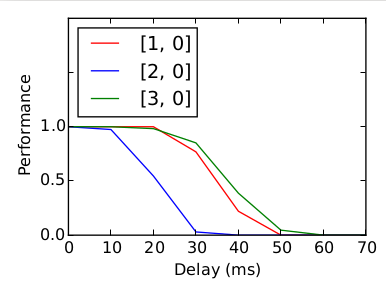
\includegraphics[width=0.45\textwidth]{PD1.png}} 
   & \subfloat[Cue shape appearing with delay - 1]{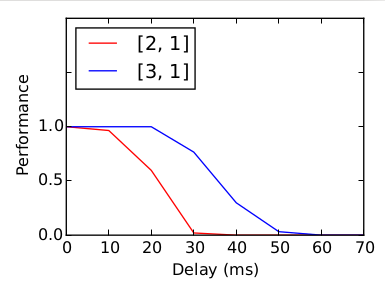
\includegraphics[width=0.45\textwidth]{PD2.png}}\\
\subfloat[Cue shape appearing with delay - 2]{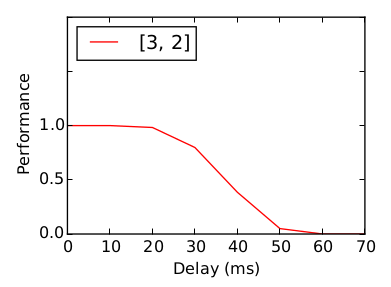
\includegraphics[width=0.45\textwidth]{PD3.png}} 
\end{tabular}
&
\end{tabularx}
\caption[Delay in second cue presentation]{Delay in second cue presentation, performance of the \emph{model}. [0,1,2,3] represent cue shapes in the decreasing order of reward probabilities [1.0,0.66,0.33,0] respectively. The \emph{model} is allowed to learn in its original state. Then each combination of the following cue pairs are presented with the more rewarding cue appearing after a delay, for 120 trials and the performance is measured. (a) 3 combinations of cue shapes with cue shape - 0 appearing after a delay in all the cases. Performance starts to decrease as cue 0 is presented after a delay grerater than 10 ms. (b) 2 combinations with cue shape 1 appearing after a delay. Performance starts to decrease after the delay is greater than 20 ms. Similar observation with the cue shape 2 presented after a delay, (c).}
\end{center}
\end{figure}

\subsection{Visual salience of the cue}
The \emph{model} encodes the visual salience of the cue shape presented as $I_{Ext}$ in the neuronal equation (Eq. 1). $I_{Ext}$ is unchanged throughtout the learning process. After the \emph{model} has learnt, change in such salience of the cue shape affected the performance of the \emph{model}. In similar terms as \emph{Section 3.2} , the \emph{model} is allowed to learn for 120 trials. In a trial when two randomly chosen cue shapes are presented simultaneously, but the lesser rewarding cue has more salience than what the \emph{model} has learnt, it is expected that the model still selects the best rewarding cue.\par
\begin{figure}[!hb]
\begin{center}
\begin{tabularx}{\linewidth}{@{}cXX@{}}
\begin{tabular}{cc}
\subfloat[Cue with lesser salience - 0]{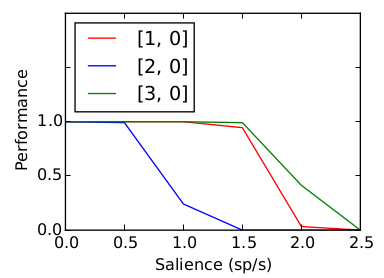
\includegraphics[width=0.45\textwidth]{PS1.png}} 
& \subfloat[Cue with lesser salience - 1]{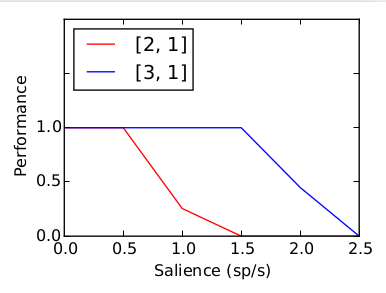
\includegraphics[width=0.45\textwidth]{PS2.png}} \\
\subfloat[Cue with lesser salience - 2]{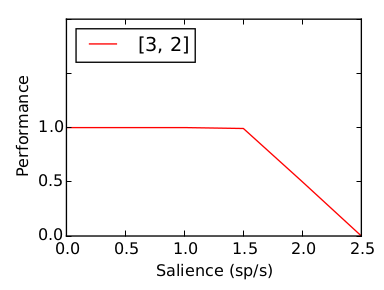
\includegraphics[width=0.45\textwidth]{PS3.png}} 
\end{tabular}
\end{tabularx}
\caption[Cue shapes with different salience]{Cue shapes with different salience, performance of the \emph{model}. [0,1,2,3] represent cue shapes in the decreasing order of reward probabilities [1.0,0.66,0.33,0] respectively. The \emph{model} is allowed to learn in its original state. Then each combination of the following cue pairs are presented.  In a trial, both the cues appear simultaneously, but the lesser rewarding cue is presented with increase in salience, for 120 trials and the performance is measured. (a) 3 combinations of cue shapes with cue shape - 0 with an increased salience to the lesser rewarding cue shape. Performance starts to decrease as the salience of the cue shape other than 0 is increased by more than 1 sp/s. (b) 2 combinations with cue shape 1 and the lesser rewarding cues with increased salience. Performance starts to decrease as the salience of the cue shape other than 1 is increased by more than 1.5 sp/s. Similar observation with the cue shape 3 presented with increased salience against cue shape 2 (c).}
\end{center}
\end{figure}
In each of the 6 pairwise cue combinations, the salience of the lesser rewarding cue shape is increased and each combination is presented for 120 trials. The performance of the \emph{model} is measured, expecting the \emph{model} still selects the best rewarding cue shape. However, the performance of the \emph{model} is observed to be reduced when the lesser rewarding cue shape is presented with a certain increase in salience. Interestingly, the increase of salience after which the \emph{model} performance decreases for each combination depends on the best rewarding cue shape in the combination. 

\section{Progress}
\subsection{As on 21/08/2015}
\textbf{\emph{Scaling}}: The results of the developments as in the section 3 give some useful insights into various factors involving decision making. However, one of the major limitations of the \emph{model} is the discrete representation of stimuli in the discussed areas. One neuron (channel) representing each cue shape stands too simplified a representation and limits us from analyzing cases like ambiguous cue shapes. With the idea of scaling up the model and have a number of neurons representing each stimulus, we decide to implement the exact model using \emph{Distributed Asynchronous Numerical \& Adaptive computing framework (DANA\footnote{http://dana.loria.fr/doc/index.html})} and then scale up the number of neurons representing the cue shape inputs in important areas of cortex and striatum.\par
Having a population of neurons representing each cue shape input, the is analyzed to find an appropriate method. A guassian input at the center of each popualation for a particular cue shape is tried, to begin with. It'll be explored how the \emph{model} translates this kind of stimuli representation to further levels in decision making.  \par
\textbf{\emph{DANA}} provides a sophisticated and simpler framework to project connections between structures of unequal populations. Also, being a python based framework, the internal representations used in \emph{DANA} helps faster computation, particularily for dynamically changing neural populations, than numpy.
\par
We have begun to convert the existing \emph{model} to \emph{DANA}. The idea is to retain the exact details of structures in the existing \emph{model} and make sure similar results are replicated; then expand the number of neurons in cortex and striatum. Owing to the knowledge that number of neurons in cortex is bigger than that in striatum, it is chosen to attempt the scaling up intially in cortex, beginning with 512 neurons in total while the projection remains to be onto 4 neurons in striatum. As the desired results are replicated, it would be fairly easy to scale up striatum.\par
\subsection{As on 04/09/2015}
The model is converted to \emph{DANA}, with structures connected through DANA connections. It is configurable to increase the population in cortex or striatum as needed. However, with increased population in cortex, the model needs to replicate the trial behaviour as exhibited in the Guthrie \emph{model} (Fig. 2)  \par
\textbf{\emph{Input}} is represented by a gaussian, over the population representing each cue shape, with mean being at the center of the population. Unlike the simplistic case in the previous \emph{model}, where a single neuron receives external current, for each cue shape, now the input is distributed across a population. Hence at the target structure, the gains need to be changed. The population in the cortex representing each cue shape (and each motor direction) is increased to 16 from 1 and that of striatum remaining 1.
\par
The sigmoidal behaviour of the cortex(cognitive and motor) activity within the first 500 ms (settling time of the trial), which is a very significant feature of the Guthrie \emph{model}, is reproduced. However the later stabilization of the activity representing both the cues, with higher activity implying selection of a choice, is not observed.
\begin{figure}[!ht]
\begin{center}
\begin{tabularx}{\linewidth}{@{}cXX@{}}
\begin{tabular}{cc}
\subfloat[Cortex activity in a trial - 1 neuron per cue shape]{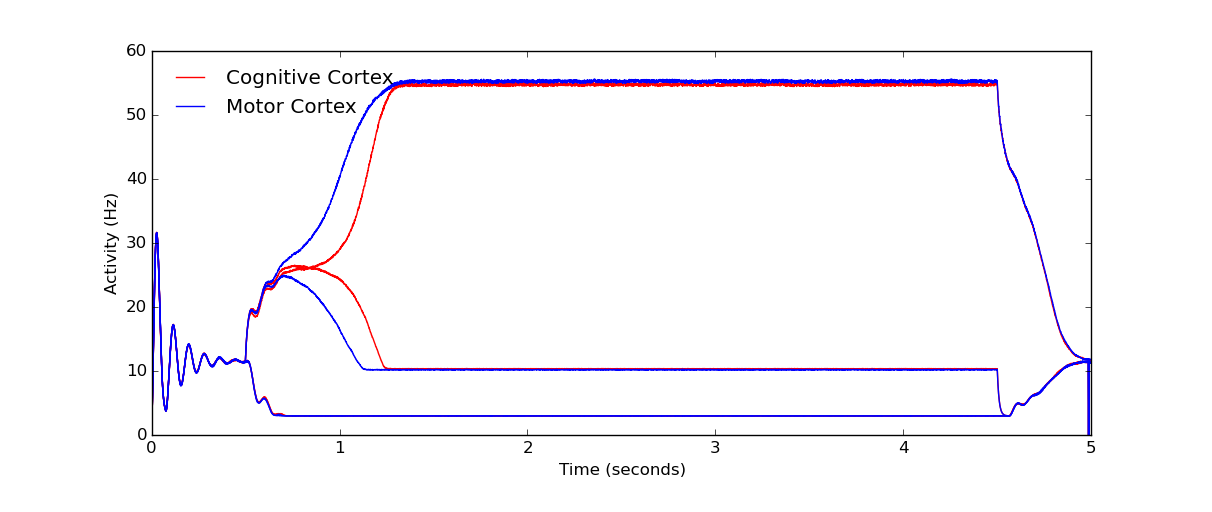
\includegraphics[width=0.85\textwidth]{trial_dana_1.png}} 
\\
\subfloat[Cortex activity in a trial - 16 neurons per cue shape]{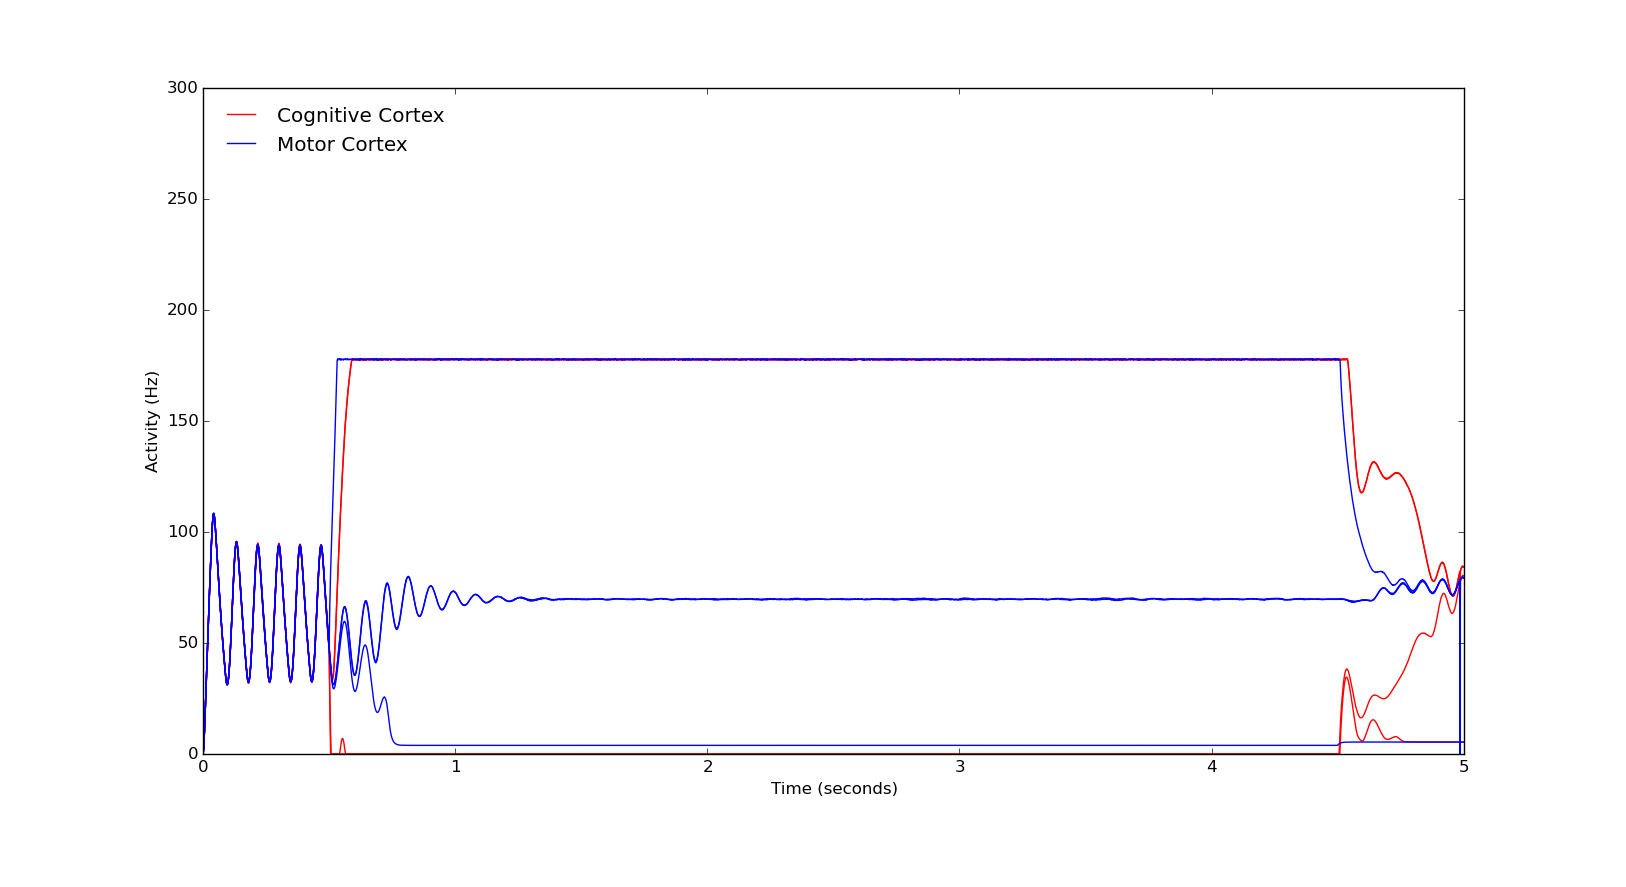
\includegraphics[width=0.85\textwidth]{trial_dana_16.png}}
\end{tabular}
\end{tabularx}
\caption[Cortex activity in each trial]{Cortex activity in each trial. With the model implemented in \emph{DANA}, and the population remaining same as the Guthrie \emph{model}, the activity cab seen as identical to that of in the Guthrie \emph{model} (a). When the the population is increased in cortex, the acitivity before the introduction of stimulus is identical. However, to obtain a selection of action, appropriate gains are to be identified.}
\end{center}
\end{figure}

\textbf{\emph{TBD - following week}} Identify suitable gains for the cortex to striatum projections, so that action selection can be observed, with a higher population in cortex to that in striatum.

\subsection{As on 11/09/2015}
\emph{\textbf{Highly populated cortex}} With a cortex population of 1024 neurons in total, together representing all the four possible cue shapes, striatum and other structures have been maintained at a population of 4 neurons, one neuron per cue shape. Some modifications have been done in the inter-structure connectivity and an increased external current is given to cortex (represent visual salience of the stimulus) but distributed normally across the population of neurons representing a stimulus.
\par Interestingly, the activity pattern after the trial in cortex, is quite similar to that of the \emph{model} at its simplest form (one neuron per each cue at every structure).

\begin{figure}[!ht]
\begin{center}
\begin{tabularx}{\linewidth}{@{}cXX@{}}
\begin{tabular}{cc}
\subfloat[Cortex activity in a trial - 256 neurons per cue shape]{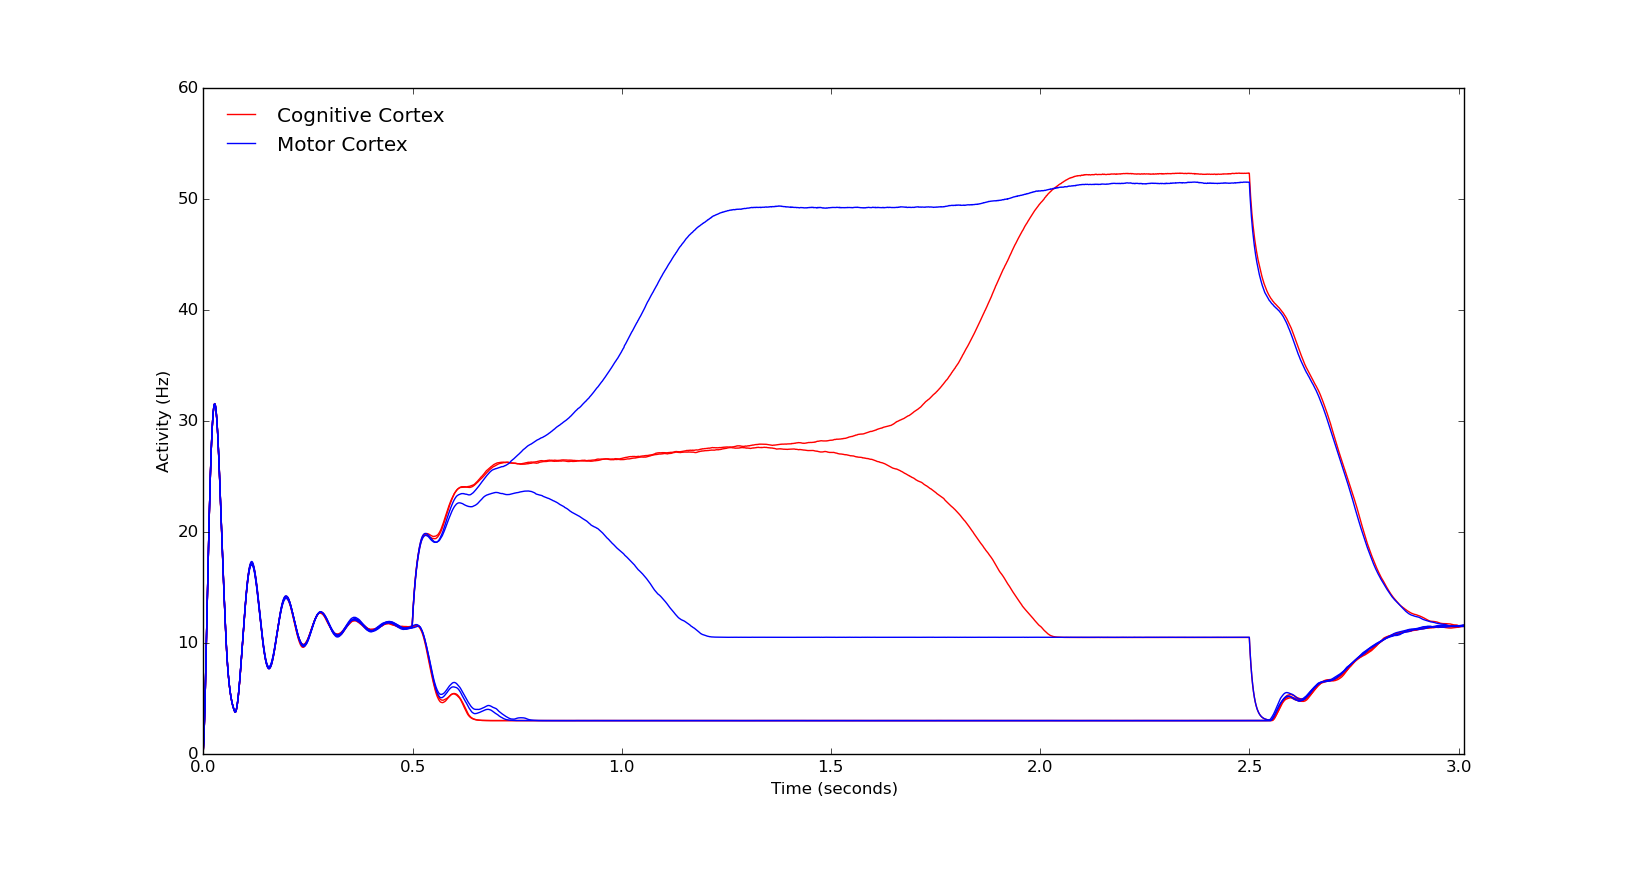
\includegraphics[width=0.85\textwidth]{cortex_activity_1024.png}} 
\\
\subfloat[Cortex - External input (trial start) \& Activity (trial end) ]{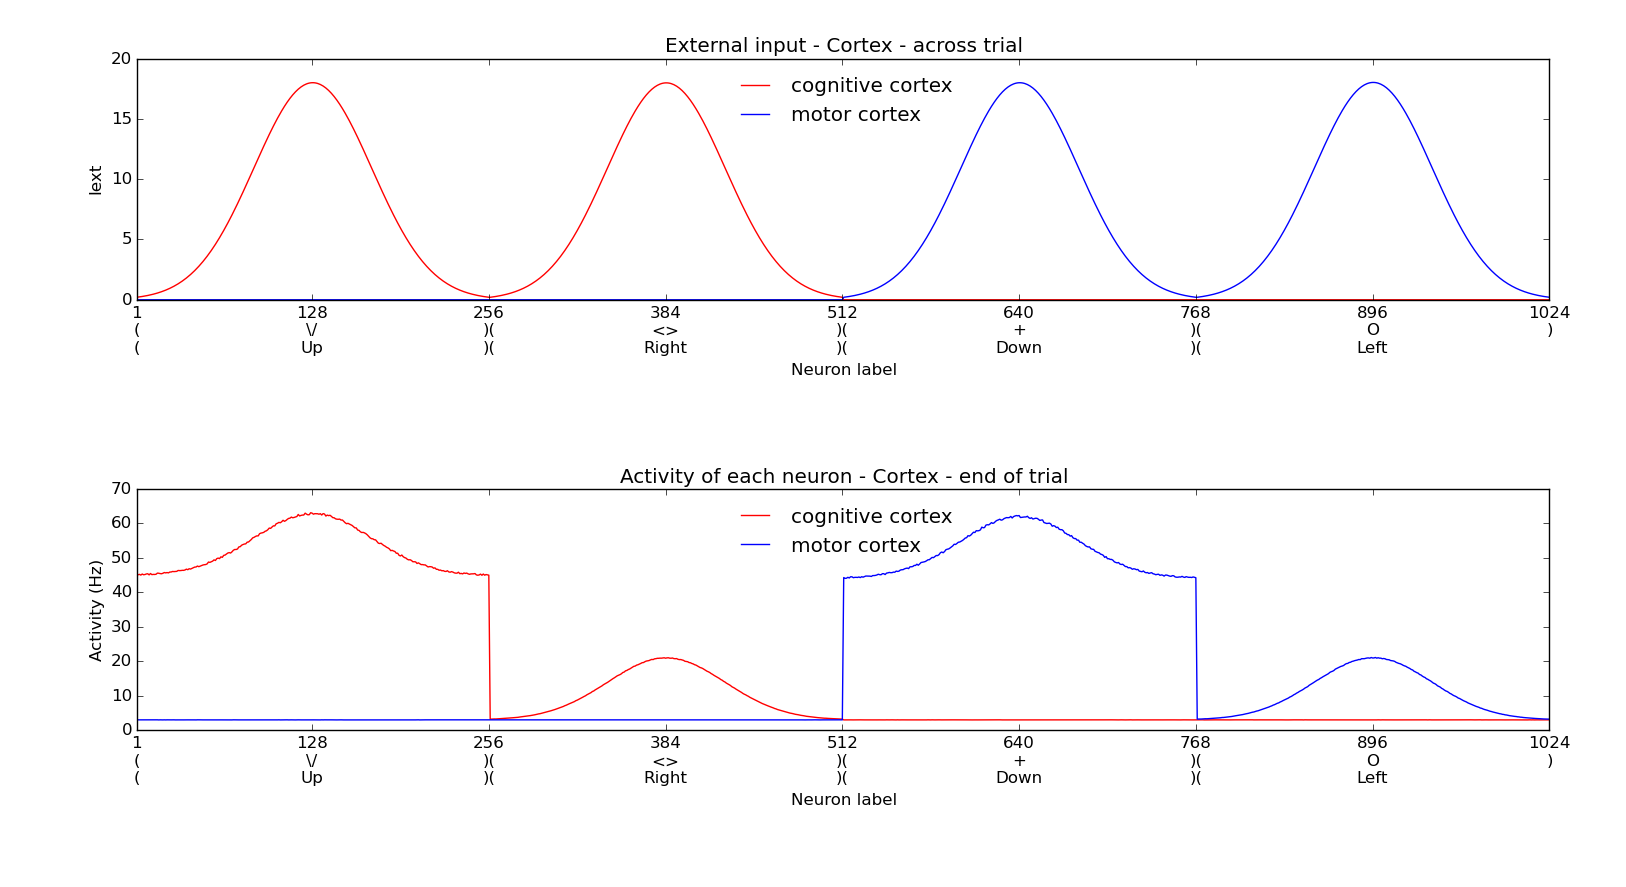
\includegraphics[width=0.85\textwidth]{input_output_1024.png}}
\end{tabular}
\end{tabularx}
\caption[Cortex activity in each trial]{Cortex activity in each trial. With 256 neurons representing each cue shape, and the mean of the final activities of each such population plotted against trial time. Similar to Fig.9(a). (b) With two gaussian external inputs each for cognitive cortex (two shapes) and motor cortex ( two positions), the activity in cognitive and motor cortex after the end of trial. }
\end{center}
\end{figure}

\par \emph{However} it is observed that 1024 neurons in cortex significantly increases the computational complexity of the model, in its current scope.
With a cortex population of 256 neurons (64 neurons per cue shape), the model exhibits similar behaviour. It is interesting to see how the model behaves if striatum is also scaled up to more than one neuron per cue shape.

\textbf{\emph{TBD - following week}} With cortex population at 256 neurons (in each of cognitive and motor channels) representing all four cue shapes (and positions), Striatum will be expanded, to 16 neurons or more in total and then observe how the model behaves.

\subsection{As on 09/10/2015}
The \emph{model} has been scaled up to a population of 256 neurons in cortex and 16 neurons each for each of the other structures. The connectivity between the structures remains similar to that in the original model, but scaled according to the increased populations. An example of such connectivity (64 neurons in cortex, 16 in other structures) can be seen in Fig.11.
\par
The \emph{model} is allowed to learn over 120 trials. Learning happens on the weights connecting the cognitive part of cortex and striatum. In each trial, depending on the cue shape decision, all the weights connecting the neurons representing particular shape are modified. 
\par
The \emph{model} is observed to reach a performance of ~0.90 at the end of 120 trials. The expanded model is very slow compared to the basic model, which makes it difficult to run 250 simulations to mearsure the overall performance of the model.
  
\textbf{\emph{TBD - following week}} The goal is to make the model run faster, so that multiple simulations can be run to measure how consistently model performs. We plan to move the structures to cython based implementation to achieve faster results. 

\clearpage
\section{Expanded model}
\subsection{Structures}
In the simplistic model, in a regular structure, there is one neuron representing each stimulus (stimulus - cue shape in a cognitive channel, cue position in a motor channel) and an associative structure has a 2D array of neurons where no. of rows and columns both equal to the no. of stimuli. Now, we move to an expanded version where a population of neurons together represent all the stimuli. To start with, we have a clear distinction in such population that each stimulus is represented by a subgroup of neurons and each subgroup with equal number of neurons. For example, in a cognitive channel of a structure, a population of 4N neurons (N>1) for 4 cue shapes, a subgroup of N neighboring neurons represent each cue shape. 

In comparison to the simplistic model, the regular (cognitive and motor channels) and associative structures are described in the following way:
\\
\par
\textbf{\emph{(Regular) Structure}}:
A 1-d array of n=4N neurons, representing 4 stimuli (cue shape or cue position). Stimulus S\textsubscript{i}  is represented by neurons \{\emph{i*N+0, i*N+1,\ldots, i*N+N-1}\}. To provide an external input corresponding to the stimulus S\textsubscript{i} in a structure, a Gaussian input is given, with mean being the center of the neurons [ i*N \textbf{:}  i*N+N-1] and sigma such that the input is almost zero towards the end neurons of this subgroup (i*N and  i*N+N-1).
\\
\par
\textbf{\emph{Associative Structure:}}:
A 2-d array of n x n (n=4N) neurons, representing the conjunction of both cognitive and motor channels with rows representing cognitive stimuli (shapes) and columns representing motor stimuli (positions). So, an input in the associative structure, (C\textsubscript{i} , M\textsubscript{j}) is represented by the subgroup of neurons [i*N \textbf{:} i*N+(N-1), j*N \textbf{:} j*N+(N-1)]. To provide an external input corresponding to the stimuli (C\textsubscript{i} , M\textsubscript{j}), a 2D Gaussian is given, with mean being at the center of the subgroup i.e, 
[i*N+p \textbf{:} i*N+p+1, j*N+p \textbf{:} j*N+p+1], where p = Ceil(N-1/2) and sigma such that the input is almost zero towards the end neurons of the subgroup - [( i*N, j*N), ( i*N, j*N+N-1), ( i*N+N-1, j*N),  ( i*N+N-1, j*N+N-1)]

\begin{figure}[h]
\begin{center}
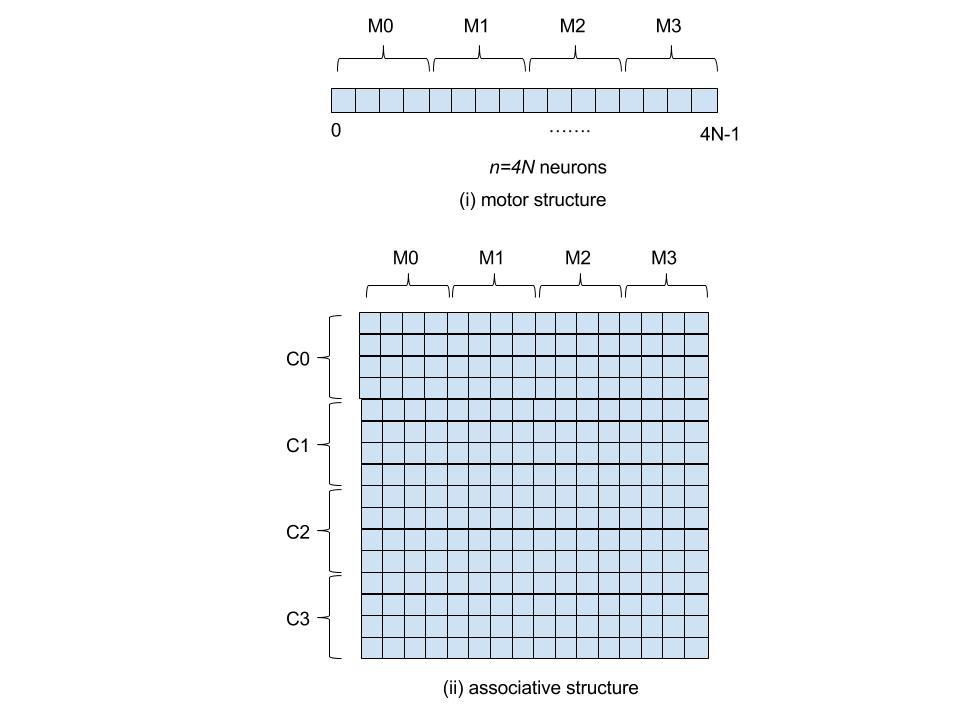
\includegraphics[width=0.85\textwidth]{Associative.jpg}
\caption[Structures]{(i) A motor structure with 4N neurons, with each N neurons representing a motor simulus (cue position). A cognitive channel also has similar structure. (ii) An associative structure with 4Nx4N (16x16 in this case) neurons. All the columns of neurons represent 4 motor stimuli equally and all rows represent the 4 cognitive stimuli.}
\end{center}
\end{figure}

\subsection{Connectivity}
Between such structures, the connectivity is based on the assumption that the neurons in both the structures are in some way labeled, belonging to particular stimuli (shape or position). It might be biologically implausible to assume such a distinct connectivity between the structures but it provides a good understanding of expanding this kind of models from simplistic implementations to complex highly populated networks. Depending on the structures in the model, we define two classes of connectivity. Two dimensional structures, viz., associative cortex, associative striatum are connected with, what we describe as Block-Connectivity. Stripe-Connectivity comprises of those connections involving the remaining one dimensional structures such as cognitive cortex to cognitive striatum, motor striatum to motor GPi etc.  

It is assumed that all the populations represent four stimuli (cue shape or position). Each connection
is between a \emph{source} and a \emph{target} structure.
\par
\subsubsection{Stripe-Connectivity} 
\textbf{\emph{One to One}} : If both source and target have same no. of neurons, every neuron in target is connected to the corresponding neuron in source. But, if the number of neurons in source and target is different: 
\begin{itemize}
  \item source - m neurons
  \item target - n neurons (n = 4N, m = kn, {N,k} >= 1)
\end{itemize}  
  \emph{neuron} i in target is connected to neurons {k*i, k*i+1,\ldots,k*i+k-1} in the source, where m = k*n.
\begin{figure}[h]
\begin{center}
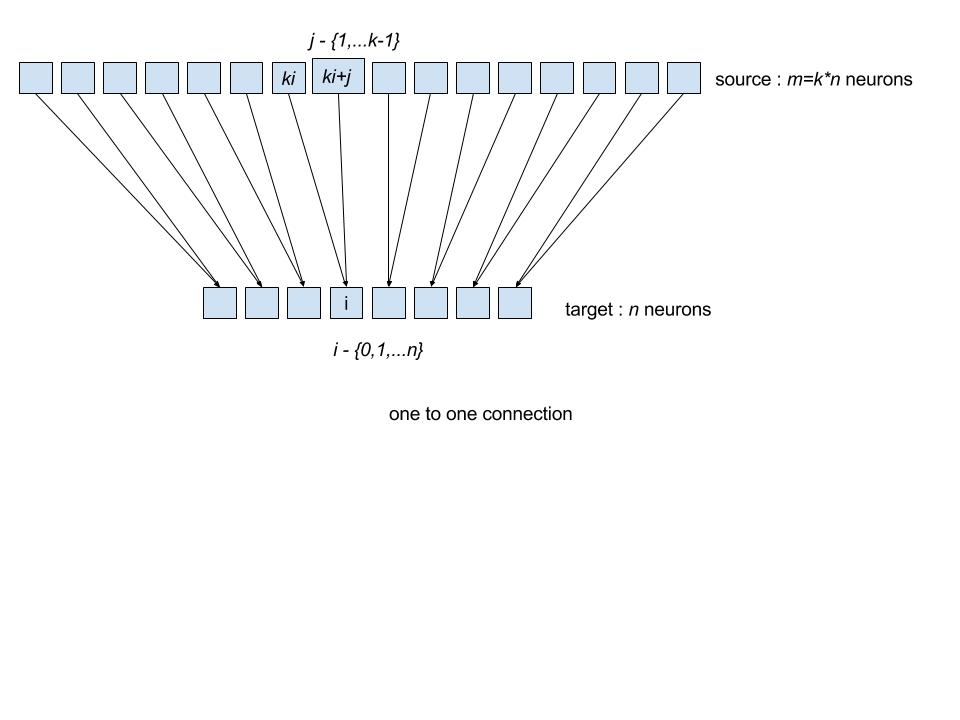
\includegraphics[trim={0 10cm 0 0},clip,width=0.85\textwidth]{OnetoOne.jpg}
\caption[One to One connectivity]{When there are \emph{n} neurons in target and \emph{m (= k * n)} neurons in the source, every neuron \emph{i} in target is connected to neurons \{k*i, k*i+1, \ldots, k*i+k-1\}.}
\end{center}
\end{figure}
\\
\par
\textbf{\emph{Regular to Associative and vice-versa}} : This kind of connectivity includes connections like cognitive cortex to associative striatum, motor cortex to associative striatum, associative striatum to cognitive GPi and associative stratum to motor GPi. Consider the following connection:
\begin{itemize}
  \item source - regular structure, m neurons , m=k*n (k>1)
  \item target - associative structure, n x n neurons
\end{itemize}  

Every neuron \emph{i} in source is connected to neurons [Quotient(i,k), \textbf{:}] (\emph{Quotient(a,b) - quotient when a is divided by b})in the target, which implies each neuron in cognitive cortex is connected to the neurons representing all the motor stimuli and the corresponding cognitive stimulus. And in the similar way, if the source is motor cortex, every neuron \emph{i} is connected to neurons [\textbf{:}, Quotient(i,k)] in the target implying each neuron in motor cortex is connected to the neurons representing all the cognitive stimuli and the corresponding motor stimulus in associative striatum. 
	Similar connectivity can be extended conversely to other connections involving associative striatum, such as associative striatum to cognitive GPi and associative striatum to motor GPi. 
\\
\\
\\
\begin{figure}[ht]
\begin{center}
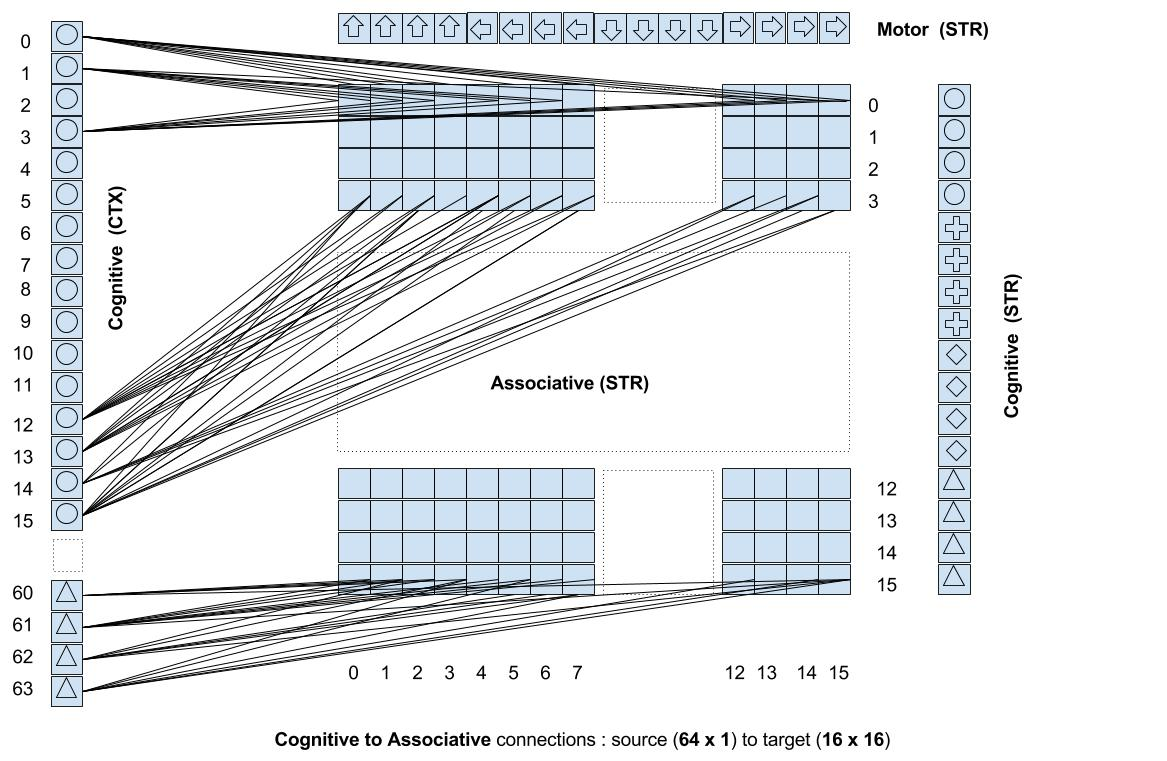
\includegraphics[width=0.85\textwidth]{CogToAssociative.jpg}
\caption[Cognitive (cortex) to Associative (striatum)]{Connectivity between cognitive structure of cortex and the associative structure of striatum. The cognitive cortex neurons representing each shape are connected to all the neurons corresponding to the same shape in the associative striatum including all the possible directions. In this case, when cortex has a total of 64 neurons for the cognitive part and striatum has 16 each for cognitive and motor part (hence, a 16x16 associative part)}
\end{center}
\end{figure}

\subsubsection{Block-Connectivity}
\textbf{\emph{Associative to Associative connection}} : 
\begin{itemize}
  \item source - Associative structure, m x m neurons (m = k*n)
  \item target - Associative structure, n x n neurons (n = 4N, {N,k} >= 1)
\end{itemize}  

In this connection, in each associative structure, only those neurons corresponding to stimulus S\textsubscript{i} - [C\textsubscript{i} , M\textsubscript{i}] (0<=i<=3) have connections. For example, in the target structure, any neuron (i,j) has a connection if only if :
i $\epsilon$ [p*N \textbf{:} p*N+N-1] and j $\epsilon$ [p*N \textbf{:} p*N+N-1] for some p >= 0

Between the source and target, only the neurons representing same stimulus (C\textsubscript{i} , M\textsubscript{i}) are connected. Assuming target has n x n neurons and source has kn x kn neurons, neuron (i,j) in target is connected to a \textbf{block b} of neurons in the source \\

\textbf{b} - [k*i \textbf{:} k*i+k-1, k*j \textbf{:} k*j+k-1] 

\begin{figure}[h]
\begin{center}
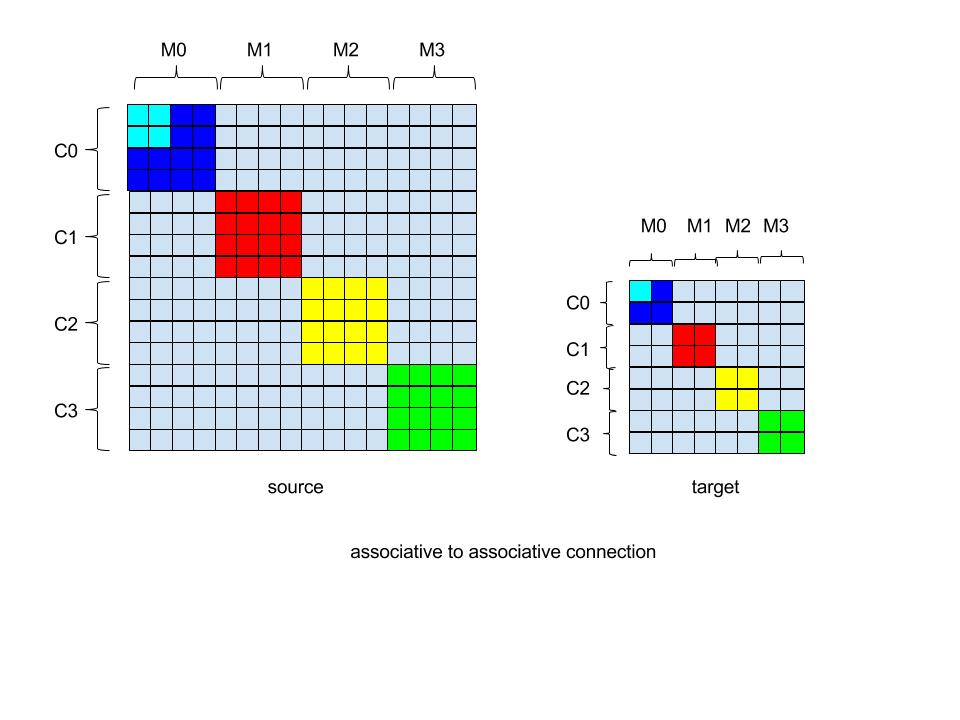
\includegraphics[width=0.85\textwidth]{AssociativeToAssociative.jpg}
\caption[Associative (cortex) to Associative (striatum)]{Neurons corresponding to each stimulus in both the structures are connected. For a given stimulus (C\textsubscript{0} , M\textsubscript{0}), each neuron in target is connected to a block of neurons in source. For eg, neuron (0,0) in target is connected to the block [(0,0,(0,1),(1,0),(1,1)] in source. Similarly all the neurons that are connected are highlighted in colors.}
\end{center}
\end{figure}
	
\subsection{Working Model}
Using the above described structures and connections, we build a large computational model, which exhibits the intrinsic functional properties of \emph{Guthrie's model} but significantly higher number of neurons in each structure and hence more complex stimulus representations and decision making process. The population of structures and the connections among them are listed in \textbf{Table 1} and \textbf{Table 2}.
\begin{table}
\centering
\begin{tabular}{l*{6}{c}r}
Structure         &  & Channel &  & Total \\
\hline
         & cognitive & motor & associative &  \\
\hline
Cortex   & 256 & 256 & 65536 & 66048  \\
Striatum &  16 &  16 &   256 &   288  \\
GPi      &  16 &  16 &   -   &    32  \\
Thalamus &  16 &  16 &   -   &    32  \\
STN      &  16 &  16 &   -   &    32  \\
\hline
         &     &     &       & 66432 neurons \\
\hline
\end{tabular}
\caption{No. of neurons in each structure}\label{table:model}
\end{table}

\begin{table}
\centering
\begin{tabular}{l*{6}{c}r}
Connection         &  Source  & Target \\
\hline
One to One                   & cognitive cortex & cognitive striatum  \\
One to One                   & motor cortex     & motor striatum  \\
Associative to Associative   & associative cortex & associative striatum  \\
Cognitive to Associative     & cognitive cortex & associative striatum  \\
Motor to Associative         & motor cortex & associative striatum  \\
One to One                   & cognitive cortex & cognitive STN  \\
One to One                   & motor cortex     & motor STN  \\
One to One                   & cognitive striatum & cognitive GPi  \\
One to One                   & motor striatum     & motor GPi  \\
Associative to Cognitive     & associative striatum  & cognitive GPi  \\
Associative to Motor         & associative striatum  & motor GPi  \\
One to All                   & cognitive STN & cognitive GPi  \\
One to All                   & motor STN     & motor GPi  \\
One to One                   & cognitive GPi & cognitive thalamus  \\
One to One                   & motor GPi     & motor thalamus  \\
One to One                   & cognitive thalamus & cognitive cortex  \\
One to One                   & motor thalamus     & motor cortex  \\
One to One                   & cognitive cortex & cognitive thalamus  \\
One to One                   & motor cortex     & motor thalamus  \\
\hline
\end{tabular}
\caption{Connections among structures}\label{table:connections}
\end{table}

\subsection{Results}
The expanded model, as described in \emph{Table 1} and \emph{Table 2} is coded in both DANA and cython. The \emph{Associative to Associative} connection between cortex and striatum is computationally quite expensive and limits the model to run faster. With an added simplification in the way this particular connection is processed, there is a huge gain in processing time. And the expanded model could successfully take a decision in a trial (\emph{Fig. 15}), learn based on reward and achieve a performance of around \emph{0.85}
\begin{figure}[h]
\begin{center}
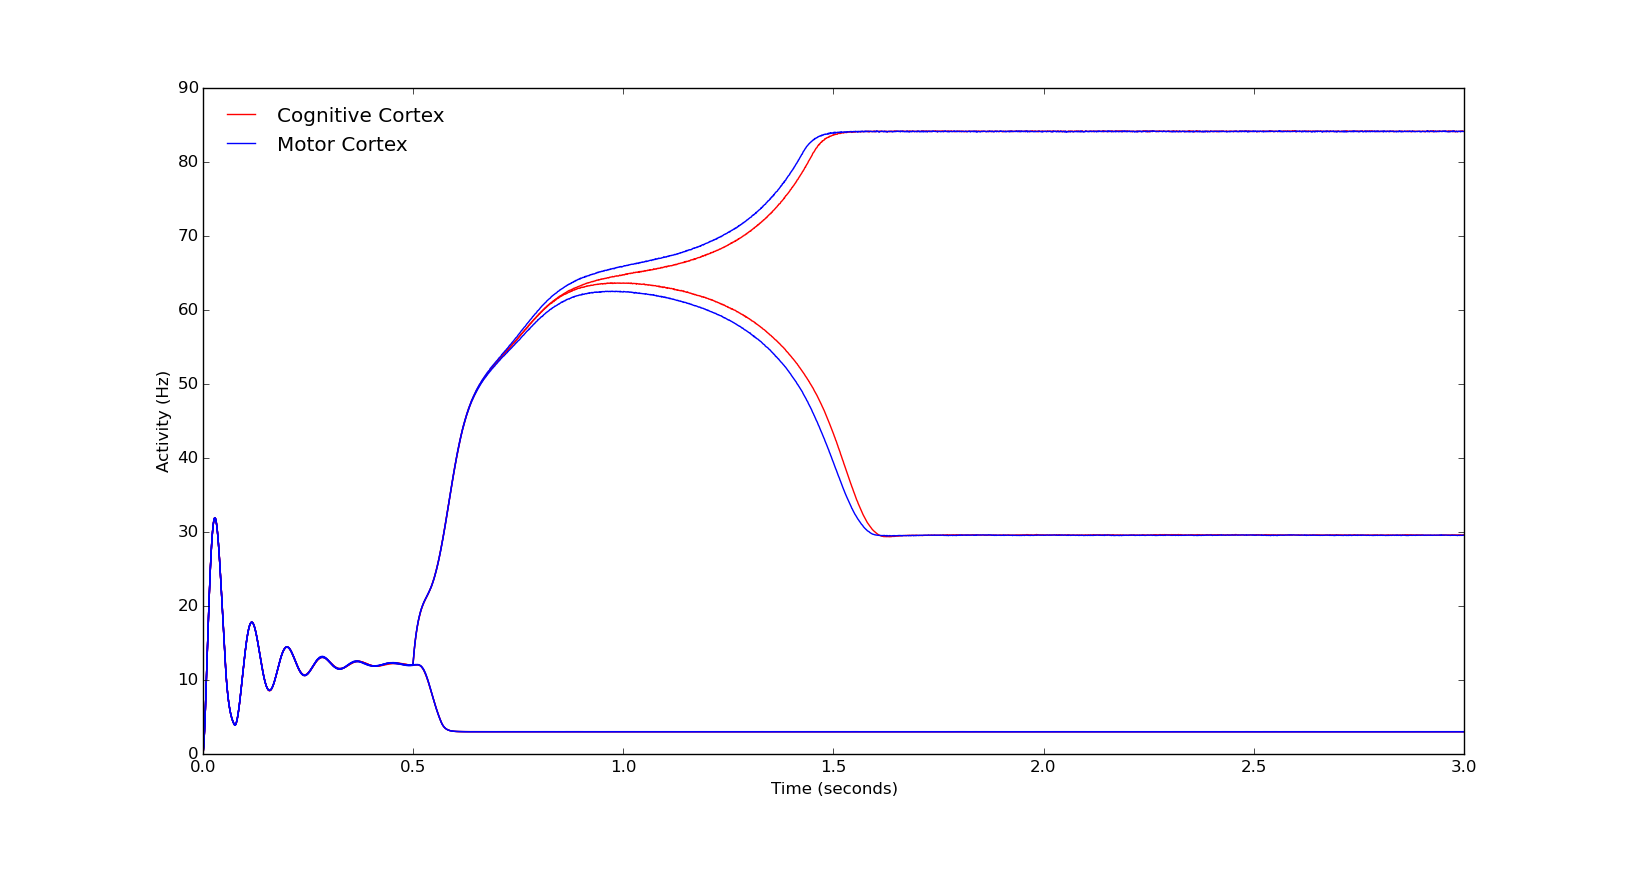
\includegraphics[width=0.85\textwidth]{cython_large_trial.png}
\caption[Expanded model, Activity of cortex, cognitive and motor channels.]{The activity of cognitive and motor cortex through the trial. Assuming certain subgroup of neurons represent certain stimulus, the activity is averaged over the subgroup and is plotted for each stimulus. It can be observed that there is decision taken for only one stimulus in both cognitive and motor channels.}
\end{center}
\end{figure}

\textbf{\emph{TBD the following week(s)}} : One of the limitations of the expanded model is that the neurons are assumed to be subgroups representing certain stimulus. Hence, the external input representation translates to giving input to such subgroups in particular.  But we desire to represent external input as a gaussian input in continuous pattern rather than discretly giving to a particualr subgroup of neurons. This also extends to the connections between the structures. Instead of connecting certain subgroup of neurons in both the structures for each stimulus, connections need to be more uniform across the structures.   
\clearpage
\nocite{*}
\bibliography{decisionmaking.bib}{}
\bibliographystyle{plain}

\end{document}